\documentclass[10pt, a4paper]{scrartcl}

\usepackage{vorschule}
\usepackage[
    typ=ab,
    fach=Informatik,
    lerngruppe={IF-EF},
    nummer=1,
    module={Symbole,Lizenzen},
    seitenzahlen=keine,
    farbig,
    lizenz=cc-by-nc-sa-4,
]{schule}

\usepackage[
	kuerzel=Ngb,
	reihe={Objektorientierte Programmierung},
	version={2020-08-31},
]{ngbschule}

\author{J. Neugebauer}
\title{Greenfoot}
\date{\Heute}

\setzeAufgabentemplate{ngbnormal}

\begin{document}

\ReiheTitel

\vspace{1.5cm}
\begin{tikzpicture}[red color/.style={draw=red!80!black,line width=2pt},marker/.style={red color,fill=red!50!black,fill opacity=.2},red circle/.style={marker,circle,minimum width=1cm,minimum height=1cm},red rect/.style={marker},red rect/.style={marker,rectangle,minimum width=1cm,minimum height=1cm,rounded corners=1pt},text field/.style={},red line/.style={red color}]
	\node[] (screen) at (0,0) {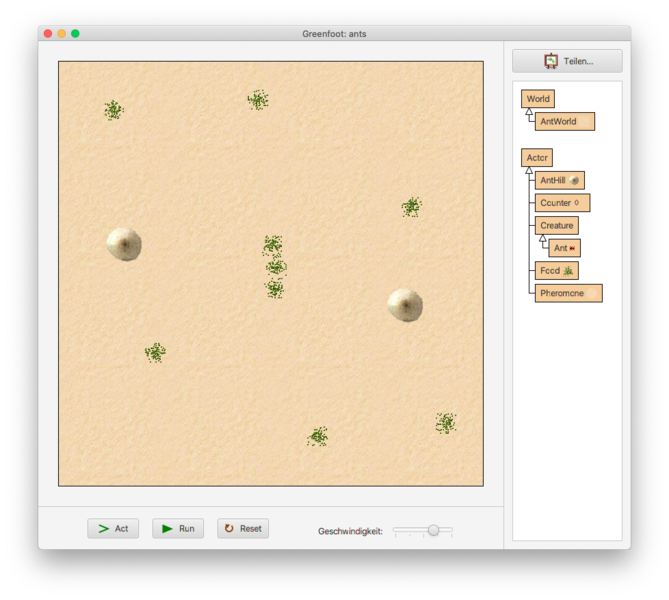
\includegraphics[width=14cm]{EF-AB.1-Abb_Ants}};


	\node[red circle] (actBtn) at (-4.6,-4.8) {};
	\node[minimum width=4cm] (actText) at (-7.2,-5.8) {};
	\draw[red line] (actText.south west) -- (actText.south east) -- (actBtn);

	\node[red circle] (runBtn) at (-3.2,-4.8) {};
	\node[minimum width=4cm] (runText) at (-5.6,-7) {};
	\draw[red line] (runText.south west) -- (runText.south east) -- (runBtn);

	\node[red circle] (resetBtn) at (-1.9,-4.8) {};
	\node[minimum width=4cm] (resetText) at (0.6,-7) {};
	\draw[red line] (resetBtn) -- (resetText.south west) -- (resetText.south east);

	\node[red rect,minimum width=1.8cm,minimum height=.6cm] (speedSlider) at (1.85,-4.8) {};
	\node[minimum width=4cm] (speedText) at (5.8,-6) {};
	\draw[red line] (speedSlider) -- (speedText.south west) -- (speedText.south east);

	\node[red rect,minimum width=9cm,minimum height=9cm] (world) at (-1.35,0.55) {};
	\node[minimum width=6cm] (worldText) at (-5.6,6.2) {};
	\draw[red line] (worldText.south west) -- (worldText.south east) -- (world);

	\node[red rect,minimum width=2.4cm,minimum height=5.4cm] (classList) at (4.9,2.0) {};
	\node[minimum width=4cm] (classText) at (1.8,6.2) {};
	\draw[red line] (classText.south west) -- (classText.south east) -- (classList);
\end{tikzpicture}
\vspace{1.5cm}

\begin{aufgabe}[symbol=\Large\symLaptop\yspace\symPartner]
	\begin{teilaufgaben}
		\teilaufgabe Öffne das Projekt \ordner{ants} aus dem Greenfoot-Ordner (\ordner{C:/Programme/Greenfoot/scenarios/java/ants)}) in Greenfoot.
		\teilaufgabe Probiert die Funktionen von Greenfoot aus.
		\teilaufgabe Tragt eure Entdeckungen und Vermutungen zu den Funktionen auf den Linien ein. Notiert euch gegebenenfalls weitere Stichpunkte, die die Funktion / das Element beschreiben.
	\end{teilaufgaben}
\end{aufgabe}

\end{document}
